%\VignetteEngine{knitr::knitr}
\documentclass{article}\usepackage[]{graphicx}\usepackage[]{color}
%% maxwidth is the original width if it is less than linewidth
%% otherwise use linewidth (to make sure the graphics do not exceed the margin)
\makeatletter
\def\maxwidth{ %
  \ifdim\Gin@nat@width>\linewidth
    \linewidth
  \else
    \Gin@nat@width
  \fi
}
\makeatother

\definecolor{fgcolor}{rgb}{0.345, 0.345, 0.345}
\newcommand{\hlnum}[1]{\textcolor[rgb]{0.686,0.059,0.569}{#1}}%
\newcommand{\hlstr}[1]{\textcolor[rgb]{0.192,0.494,0.8}{#1}}%
\newcommand{\hlcom}[1]{\textcolor[rgb]{0.678,0.584,0.686}{\textit{#1}}}%
\newcommand{\hlopt}[1]{\textcolor[rgb]{0,0,0}{#1}}%
\newcommand{\hlstd}[1]{\textcolor[rgb]{0.345,0.345,0.345}{#1}}%
\newcommand{\hlkwa}[1]{\textcolor[rgb]{0.161,0.373,0.58}{\textbf{#1}}}%
\newcommand{\hlkwb}[1]{\textcolor[rgb]{0.69,0.353,0.396}{#1}}%
\newcommand{\hlkwc}[1]{\textcolor[rgb]{0.333,0.667,0.333}{#1}}%
\newcommand{\hlkwd}[1]{\textcolor[rgb]{0.737,0.353,0.396}{\textbf{#1}}}%

\usepackage{framed}
\makeatletter
\newenvironment{kframe}{%
 \def\at@end@of@kframe{}%
 \ifinner\ifhmode%
  \def\at@end@of@kframe{\end{minipage}}%
  \begin{minipage}{\columnwidth}%
 \fi\fi%
 \def\FrameCommand##1{\hskip\@totalleftmargin \hskip-\fboxsep
 \colorbox{shadecolor}{##1}\hskip-\fboxsep
     % There is no \\@totalrightmargin, so:
     \hskip-\linewidth \hskip-\@totalleftmargin \hskip\columnwidth}%
 \MakeFramed {\advance\hsize-\width
   \@totalleftmargin\z@ \linewidth\hsize
   \@setminipage}}%
 {\par\unskip\endMakeFramed%
 \at@end@of@kframe}
\makeatother

\definecolor{shadecolor}{rgb}{.97, .97, .97}
\definecolor{messagecolor}{rgb}{0, 0, 0}
\definecolor{warningcolor}{rgb}{1, 0, 1}
\definecolor{errorcolor}{rgb}{1, 0, 0}
\newenvironment{knitrout}{}{} % an empty environment to be redefined in TeX

\usepackage{alltt}


%%%%%%%%%%%%%%%%
%%% Preamble %%%
%%%%%%%%%%%%%%%%

%%% Title %%%
\newcommand{\thetitle}{Kmer distance: Pairwise distance base on kmer strategy}

%%% Packages %%%
\usepackage{whbiocvignette}
\usepackage[numbers]{natbib}

%%% Title Material %%%
\title{}
\title{\textsf{\textbf{\thetitle}}}

\author{
	Cai Huang\\[1em]Georgia Instutute of Technology,\\ Atlanta, GA, USA\\ \texttt{chuang95@gatech.edu}
	\and
	Fredrik O. Vannberg\\[1em]Georgia Instutute of Technology,\\ Atlanta, GA, USA\\ \texttt{fredrik.vannberg@biology.gatech.edu}
}


%%%%%%%%%%%%%%%%
%%% Document %%%
%%%%%%%%%%%%%%%%
\IfFileExists{upquote.sty}{\usepackage{upquote}}{}
\begin{document}



%%% Title %%%
\maketitle


%%%%%%%%%%%%%%%%
%%% Abstract %%%
%%%%%%%%%%%%%%%%
\abstract

To date the comparison of genomic DNA sequences have routinely utilized shorter conserved regions for comparative genomics. Current phylogenetic analysis therefore can create divergent results based on which genetic loci are utilized for this analysis. Sequence similarity is also commonly determined by first carrying out gap penalty pairwise alignments for a set of sequences, and the similarity is quantified based upon this alignment. Here we provide a R package which has two kmer base algorithms to compute the pairwise comparison of genomic DNA sequence. First function is Boolean analysis by using XOR discrete function, second function is linear algebra analysis by using hierarchical PCA.


%%%%%%%%%%%%%%%%%%%%%%%%%
%%% Table of contents %%%
%%%%%%%%%%%%%%%%%%%%%%%%%
\tableofcontents


%%%%%%%%%%%%%%%%%%%%%%%%%%%%%
%%% Loading the R package %%%
%%%%%%%%%%%%%%%%%%%%%%%%%%%%%
\section{Loading the R package}
\label{sec.loading}

First, download and install the \Rpackage{kmerDistance} R package. Launch R and load the package.

\begin{knitrout}
\definecolor{shadecolor}{rgb}{0.969, 0.969, 0.969}\color{fgcolor}\begin{kframe}
\begin{alltt}
\hlkwd{require}\hlstd{(Matrix)}
\end{alltt}


{\ttfamily\noindent\itshape\color{messagecolor}{\#\# Loading required package: Matrix\\\#\# Loading required package: methods}}\begin{alltt}
\hlkwd{library}\hlstd{(kmerDistance)}
\end{alltt}
\end{kframe}
\end{knitrout}

The examples in this document are integer kc files generated by using Kanalyze\cite{Audano:2014aa} with following command.
\[{\rm{ls *fna | xargs  - I one java  - jar kanalyze.jar count  - k 8  - o one\_8.kc  - f fasta  - p kanalyze.outfmt = int  - r one}}\]

The kc files contents kmer and counts for each genome sequence. In our test data set, there are 6 kc files generated from 6 virus genome sequences, and we choose kmer length equal to 8

%%%%%%%%%%%%%%%%%%%%%%%%
%%% kmer distance by xor %%%
%%%%%%%%%%%%%%%%%%%%%%%%
\section{Compute pairwise distance by using XOR}
\label{kmerDistance.dif}

The first function \Rfunction{kmerDistance.dif} compute pairwise distance of kmer data by using XOR discrete function, and we call it boolean analysis. We can call this function.

\begin{knitrout}
\definecolor{shadecolor}{rgb}{0.969, 0.969, 0.969}\color{fgcolor}\begin{kframe}
\begin{alltt}
\hlstd{x} \hlkwb{<-} \hlkwd{kmerDistance.dif}\hlstd{(}\hlnum{8}\hlstd{,}\hlstr{"../../kmerDistance/data/"}\hlstd{)} \hlcom{#kmer.length = 8, path.to.data to data folder}
\end{alltt}
\end{kframe}
\end{knitrout}

The \texttt{x} return value is a distance matrix. Each column and row represents one virus genome. We can check the distance matrix.

\begin{knitrout}
\definecolor{shadecolor}{rgb}{0.969, 0.969, 0.969}\color{fgcolor}\begin{kframe}
\begin{alltt}
\hlkwd{names}\hlstd{(x)}
\end{alltt}
\begin{verbatim}
## [1] "Mycobacterium.phage.Phaedrus.complete.genome.fna_8.kc"
## [2] "Mycobacterium.phage.Phlyer.complete.genome.fna_8.kc"  
## [3] "Mycobacterium.phage.Pipefish.complete.genome.fna_8.kc"
## [4] "Staphylococcus.phage.55.complete.genome.fna_8.kc"     
## [5] "Staphylococcus.phage.69.complete.genome.fna_8.kc"     
## [6] "Staphylococcus.phage.71.complete.genome.fna_8.kc"
\end{verbatim}
\begin{alltt}
\hlkwd{names}\hlstd{(x)} \hlkwb{<-} \hlkwd{c}\hlstd{(}\hlnum{1}\hlopt{:}\hlnum{6}\hlstd{)}
\hlstd{x}
\end{alltt}
\begin{verbatim}
##         1       2       3      4      5      6
## 1 0.00000 0.04437 0.10764 0.6296 0.6423 0.6327
## 2 0.04437 0.00000 0.09808 0.6282 0.6429 0.6326
## 3 0.10764 0.09808 0.00000 0.6255 0.6399 0.6290
## 4 0.62958 0.62823 0.62552 0.0000 0.2745 0.2079
## 5 0.64226 0.64290 0.63994 0.2745 0.0000 0.2796
## 6 0.63266 0.63260 0.62903 0.2079 0.2796 0.0000
\end{verbatim}
\end{kframe}
\end{knitrout}

First 3 virus are \emph{Mycobacterium.phage} and last 3 are \emph{Staphylococcus.phage}. From the matrix, we see the pairwise distance among first 3 genomes and last 3 genomes are lower than the pairwise distance across the them. Base on this, we can clearly cluster them to two family.\\


%%%%%%%%%%%%%%%%%%%%%%%%
%%% kmer distance by hPCA %%%
%%%%%%%%%%%%%%%%%%%%%%%%
\section{Compute pairwise distance by using hierarchical PCA}
\label{kmerDistance.hpca}

The second function. \Rfunction{kmerDistance.hpca} compute the pairwise distance of kmer data by using hierarchical PCA, and we call it linear algebra analysis. We can call this function.

\begin{knitrout}
\definecolor{shadecolor}{rgb}{0.969, 0.969, 0.969}\color{fgcolor}\begin{kframe}
\begin{alltt}
\hlstd{y} \hlkwb{<-} \hlkwd{kmerDistance.hpca}\hlstd{(}\hlnum{8}\hlstd{,}\hlstr{"../../kmerDistance/data/"}\hlstd{)} \hlcom{#kmer.length = 8, path.to.data to data folder}
\end{alltt}
\end{kframe}
\end{knitrout}

This function also  returns \texttt{y} value as a distance matrix. Each column and row represents one virus genome. We can check the distance matrix.

\begin{knitrout}
\definecolor{shadecolor}{rgb}{0.969, 0.969, 0.969}\color{fgcolor}\begin{kframe}
\begin{alltt}
\hlkwd{names}\hlstd{(y)}
\end{alltt}
\begin{verbatim}
## [1] "Mycobacterium.phage.Phaedrus.complete.genome.fna_8.kc"
## [2] "Mycobacterium.phage.Phlyer.complete.genome.fna_8.kc"  
## [3] "Mycobacterium.phage.Pipefish.complete.genome.fna_8.kc"
## [4] "Staphylococcus.phage.55.complete.genome.fna_8.kc"     
## [5] "Staphylococcus.phage.69.complete.genome.fna_8.kc"     
## [6] "Staphylococcus.phage.71.complete.genome.fna_8.kc"
\end{verbatim}
\begin{alltt}
\hlkwd{names}\hlstd{(y)} \hlkwb{<-} \hlkwd{c}\hlstd{(}\hlnum{1}\hlopt{:}\hlnum{6}\hlstd{)}
\hlstd{y}
\end{alltt}
\begin{verbatim}
##          1        2        3       4     5       6
## 1 0.000000 0.001199 0.005339 0.92827 1.154 0.89736
## 2 0.001199 0.000000 0.005555 0.92876 1.155 0.89793
## 3 0.005339 0.005555 0.000000 0.92916 1.152 0.89808
## 4 0.928267 0.928765 0.929163 0.00000 1.260 0.07331
## 5 1.154281 1.155395 1.151979 1.25968 0.000 1.18652
## 6 0.897357 0.897929 0.898078 0.07331 1.187 0.00000
\end{verbatim}
\end{kframe}
\end{knitrout}

Similarly, we see the pairwise distance are clearly separating the two group of viruses.\\


%%%%%%%%%%%%%%%%%%%%%%%%
%%% compare the result%%%
%%%%%%%%%%%%%%%%%%%%%%%%
\section{Compare the results generated by XOR and hierarchical PCA}
\label{kmerDistance.dif}

Further more, we plot the \texttt{x} and \texttt{y} pairwise distance matrix together, and show the nice correlation between our two algorithm.

\begin{knitrout}
\definecolor{shadecolor}{rgb}{0.969, 0.969, 0.969}\color{fgcolor}\begin{kframe}
\begin{alltt}
\hlcom{#prepare the result as vector}
\hlstd{x}\hlkwb{=}\hlkwd{as.vector}\hlstd{(}\hlkwd{data.matrix}\hlstd{(x))}
\hlstd{y}\hlkwb{=}\hlkwd{as.vector}\hlstd{(}\hlkwd{data.matrix}\hlstd{(y))}
\hlcom{#log transfer data }
\hlstd{x[x}\hlopt{>}\hlnum{0}\hlstd{]}\hlkwb{=}\hlopt{-}\hlkwd{log}\hlstd{(x[x}\hlopt{>}\hlnum{0}\hlstd{])}
\hlstd{y[y}\hlopt{>}\hlnum{0}\hlstd{]}\hlkwb{=}\hlopt{-}\hlkwd{log}\hlstd{(y[y}\hlopt{>}\hlnum{0}\hlstd{])}
\hlcom{#fit a linear regression model to show the correlation between x and y }
\hlstd{reg}\hlkwb{=}\hlkwd{lm}\hlstd{(x}\hlopt{~}\hlstd{y)}
\hlkwd{plot}\hlstd{(x, y,}\hlkwc{xlab}\hlstd{=}\hlstr{"Boolean analysis"}\hlstd{,}\hlkwc{ylab}\hlstd{=}\hlstr{"hierarchical PCA"}\hlstd{)}
\hlkwd{title}\hlstd{(}\hlkwc{main}\hlstd{=}\hlstr{"Boolean analysis compare with hierarchical PCA"}\hlstd{,} \hlkwc{col.main}\hlstd{=}\hlstr{"black"}\hlstd{,} \hlkwc{font.main}\hlstd{=}\hlnum{4}\hlstd{)}
\hlkwd{abline}\hlstd{(reg)}
\end{alltt}
\end{kframe}
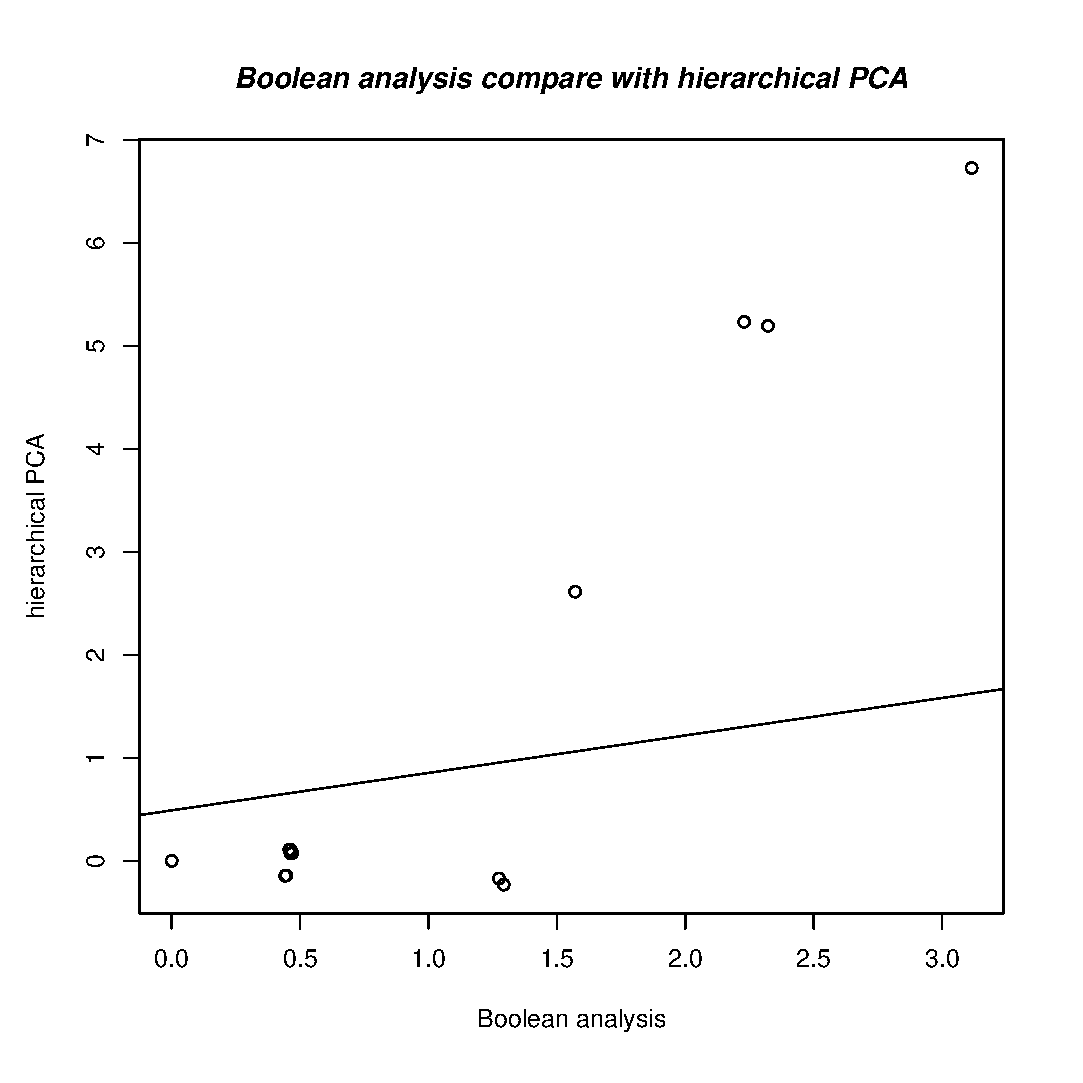
\includegraphics[width=\maxwidth]{figure/plot_result} 
\begin{kframe}\begin{alltt}
\hlcom{#show the coefficient of determination}
\hlkwd{summary}\hlstd{(reg)}\hlopt{$}\hlstd{r.squared}
\end{alltt}
\begin{verbatim}
## [1] 0.8295
\end{verbatim}
\end{kframe}
\end{knitrout}

From the plot we can see the linear regression model shows a good correlation between our two function with 0.8295 R squared score  . Also the dots are located to two separate parts of the plot, which give us the evidence of two clusters among the genome data.


%%%%%%%%%%%%%%%%%%%%
%%% Session info %%%
%%%%%%%%%%%%%%%%%%%%
\section{Session info}
\label{sec.sessioninfo}

\begin{knitrout}
\definecolor{shadecolor}{rgb}{0.969, 0.969, 0.969}\color{fgcolor}\begin{kframe}
\begin{alltt}
\hlkwd{sessionInfo}\hlstd{()}
\end{alltt}
\begin{verbatim}
## R version 3.0.3 (2014-03-06)
## Platform: x86_64-apple-darwin10.8.0 (64-bit)
## 
## locale:
## [1] en_US.UTF-8/en_US.UTF-8/en_US.UTF-8/C/en_US.UTF-8/en_US.UTF-8
## 
## attached base packages:
## [1] methods   stats     graphics  grDevices utils     datasets  base     
## 
## other attached packages:
## [1] kmerDistance_0.0.2 Matrix_1.1-4       knitr_1.6         
## 
## loaded via a namespace (and not attached):
## [1] evaluate_0.5.5  formatR_0.10    grid_3.0.3      highr_0.3      
## [5] lattice_0.20-29 stringr_0.6.2   tools_3.0.3
\end{verbatim}
\end{kframe}
\end{knitrout}

%%%%%%%%%%%%%%%%%%%%
%%% Bibliography %%%
%%%%%%%%%%%%%%%%%%%%
\bibliographystyle{natbib}
\bibliography{kmerDistance}

\end{document}
